% Provenance (never printed): cycle 4 SVT, "La planete Terre": the history of
% the Earth read in the rocks, relative dating (superposition, recoupement,
% inclusion, continuite paleontologique), the ages of the Earth, eras and
% periods, the scale of geological time; see sources/book1/PROVENANCE.md.
% Book 1, grade 7, chapter 5.
% Vocabulary guard: owns relative dating / absolute age, the four principles,
% unconformity, era and geological period, the geological time scale. The
% method of radiometric dating is the physics books' and grade 12's: told
% here in two sentences, never defined. Fossils as evidence of evolution are
% the biology books' (one sentence of prose). "Ice age" is grade 8's: not used.
\chapter{पृथ्वी के युग}\label{ch:g7:geological-time}

जून 1788 में स्कॉटलैंड के भूवैज्ञानिक जेम्स हटन और उनके दो मित्र, गणितज्ञ जॉन
प्लेफ़ेयर और रसायनज्ञ जेम्स हॉल, स्कॉटलैंड के \omterm{def:g1:landscapes-around-us:water}{तट} पर सिक्कर पॉइंट गए, एक चट्टानी
अंतरीप जिसे ``\omterm{def:g2:water-on-earth:ocean}{समुद्र} ने धो-धोकर नंगा कर दिया'' था। \omterm{def:g3:stones-pebbles-sand:rock}{चट्टान} के नीचे उन्होंने खड़ी,
लगभग ऊर्ध्वाधर धूसर परतें देखीं। उनके ऊपर लाल बलुआ पत्थर की हल्की ढलान वाली परतें
थीं। हटन ने समझाया कि क्या हुआ था: धूसर परतें किसी \omterm{def:g2:water-on-earth:ocean}{समुद्र} की तली पर समतल बिछी थीं,
फिर धकेलकर खड़ी कर दी गईं, फिर घिस गईं, और उसके बाद उनके ऊपर लाल \omterm{def:g3:stones-pebbles-sand:sand}{रेत} बिछी। इनमें से
हर चरण के लिए बहुत लंबा समय चाहिए था। प्लेफ़ेयर ने बाद में लिखा: ``समय की खाई में
इतनी दूर तक झाँकते हुए मन को जैसे चक्कर आने
लगा।''
% ledger: ncse:siccar-point

\begin{omfigure}
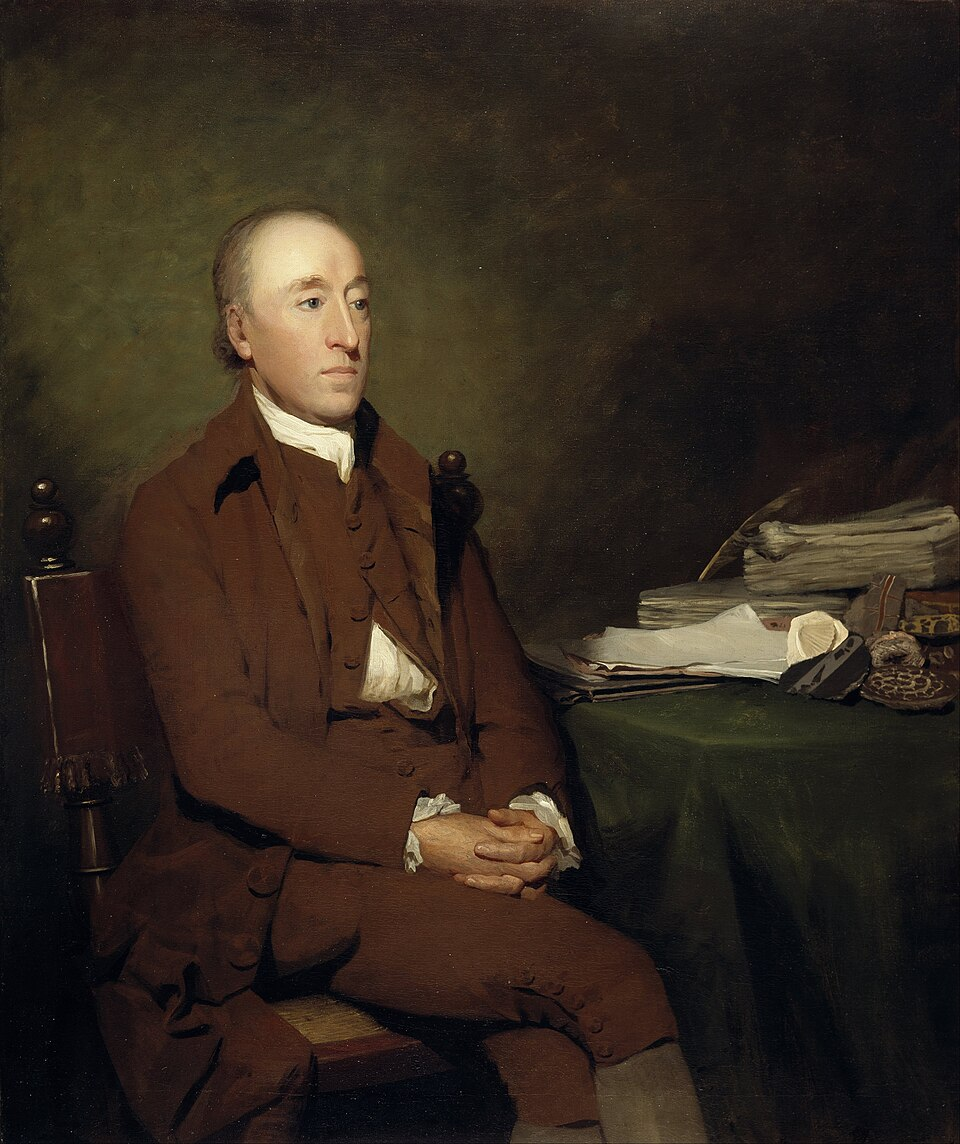
\includegraphics[width=0.3\linewidth]{images/book1/g7-hutton.jpg}

{\small जेम्स हटन (1726--1797), हेनरी रेबर्न का बनाया चित्र। हटन ने हर परत को समय
के एक हिस्से के रूप में देखा, जहाँ परतें उलटी न हुई हों वहाँ सबसे पुरानी सबसे नीचे।
चित्र सार्वजनिक डोमेन में, विकिमीडिया
कॉमन्स के ज़रिए।}
% ledger: commons:hutton-portrait, usgs:hutton-smith
\label{fig:g7:geological-time:hutton}
\end{omfigure}

बिना किसी लिखी तारीख़ के हम कैसे बता सकते हैं कि कौन-सी \omterm{def:g3:stones-pebbles-sand:rock}{चट्टान} दूसरी से पुरानी है?
पृथ्वी कितनी पुरानी है? और इतने लंबे इतिहास की कल्पना ही कैसे की
जाए?

\begin{recall}
\omterm{def:g7:sediments-and-fossils:sediment}{अवसाद} परतों में, एक के ऊपर एक, बैठते हैं और सख़्त होकर \omterm{def:g6:rocks-and-minerals:rock-families}{अवसादी चट्टान} बन जाते हैं;
\omterm{def:g7:sediments-and-fossils:fossil}{जीवाश्म} \omterm{def:g3:stones-pebbles-sand:rock}{चट्टान} में सुरक्षित जीवों के अवशेष या निशान हैं
(\cref{ch:g7:sediments-and-fossils})। \emph{\omterm{def:g7:earthquakes:fault}{भ्रंश}} \omterm{def:g3:stones-pebbles-sand:rock}{चट्टानों} में एक दरार है जिसके
साथ-साथ दोनों ओर के हिस्से खिसके हैं (\cref{ch:g7:earthquakes})। ग्रेनाइट एक
\emph{\omterm{def:g6:rocks-and-minerals:rock-families}{आग्नेय चट्टान}} है: वह तब बनती है जब पिघली \omterm{def:g3:stones-pebbles-sand:rock}{चट्टान} ज़मीन के बहुत नीचे धीरे-धीरे
ठंडी होती है; शिस्ट एक \emph{\omterm{def:g6:rocks-and-minerals:rock-families}{कायांतरित चट्टान}} है, जो ताप और दाब से बदली है;
कांग्लोमरेट आपस में सीमेंट से जुड़े \omterm{def:g3:stones-pebbles-sand:pebble}{कंकड़ों} से बनी एक \omterm{def:g6:rocks-and-minerals:rock-families}{अवसादी चट्टान} है
(\cref{ch:g6:rocks-and-minerals})।
\end{recall}

\section{पहले क्या आया?}

इतिहासकार घटनाओं को उनकी तारीख़ों के बिना भी क्रम में रख सकते हैं। पहला विश्व युद्ध
दूसरे से पहले आया: उनके नाम यही कहते हैं। जब 1903 में राइट बंधुओं ने पहली उड़ान
भरी, तब टेलीविज़न घरों में नहीं था, पर 1969 में बहुत-से लोगों ने चंद्रमा पर पहले क़दम
टेलीविज़न पर देखे: तो पहले उड़ान आई, फिर घरों में टेलीविज़न, फिर चंद्रमा। सुराग
इकट्ठे करना और उनकी तुलना करना क्रम ढूँढने के लिए काफ़ी है। पृथ्वी के लगभग पूरे
इतिहास का कोई लिखित अभिलेख है ही नहीं, और भूवैज्ञानिक इसी तरह काम करते हैं: वे
\omterm{def:g3:stones-pebbles-sand:rock}{चट्टानों} में सुरक्षित सुरागों का उपयोग करते
हैं।
% ledger: usgs:events-order

\begin{definition}[सापेक्ष काल-निर्धारण और निरपेक्ष आयु]\label{def:g7:geological-time:relative-dating}
\emph{सापेक्ष काल-निर्धारण}\index{सापेक्ष काल-निर्धारण} \omterm{def:g3:stones-pebbles-sand:rock}{चट्टानों} और घटनाओं को,
सबसे पुरानी से सबसे नई तक, क्रम में रखता है, यह बताए बिना कि वे कितने वर्ष पहले
हुईं: यह \omterm{def:g3:stones-pebbles-sand:rock}{चट्टान} उससे पुरानी है। \emph{निरपेक्ष आयु}\index{निरपेक्ष आयु} वर्षों
की संख्या के रूप में दी गई आयु है, उदाहरण के लिए
``\num{300} मिलियन वर्ष''।
\end{definition}

\section{चट्टानों को क्रम में रखने के चार सिद्धांत}

चार सरल सिद्धांत \omterm{def:g7:geological-time:relative-dating}{सापेक्ष काल-निर्धारण} का ज़्यादातर काम करते हैं। उन्हें नीचे चार
काल्पनिक खड़ी \omterm{def:g3:stones-pebbles-sand:rock}{चट्टानों} में दिखाया गया है। पहला सिद्धांत निकोलस स्टेनो ने 1669 में बताया; हटन ने अठारहवीं सदी के अंत में उस पर आगे काम किया।
% ledger: usgs:hutton-smith, og:stratigraphy-principles

\begin{omfigure}
\tikzset{
  trilo/.pic={\fill[black!65] (0,0) ellipse (0.13 and 0.085);
              \draw[white, line width=0.3pt] (-0.11,0.028) -- (0.11,0.028) (-0.11,-0.028) -- (0.11,-0.028);},
  ammo/.pic={\draw[black!75, line width=0.45pt] (0,0) circle (0.1) (0,0) circle (0.062) (0,0) circle (0.028);}
}
\begin{minipage}[t]{0.49\linewidth}\centering
\begin{tikzpicture}[font=\footnotesize]
  \fill[lith sandstone] (0,0) rectangle (4.4,0.6);
  \fill[lith shale] (0,0.6) rectangle (4.4,1.2);
  \fill[lith limestone] (0,1.2) rectangle (4.4,1.8);
  \fill[lith sandstone] (0,1.8) rectangle (4.4,2.4);
  \foreach \k in {1,2,3,4} \node[fill=white, inner sep=1pt] at (0.35,0.6*\k-0.3) {\k};
  \draw (0,0) rectangle (4.4,2.4);
  \foreach \y in {0.6,1.2,1.8} \draw[contact] (0,\y) -- (4.4,\y);
  \draw[-{Stealth}, line width=0.8pt] (4.75,0.1) -- (4.75,2.3);
  \node[anchor=west] at (4.85,2.2) {सबसे नई};
  \node[anchor=west] at (4.85,0.2) {सबसे पुरानी};
\end{tikzpicture}

{\small (क) अध्यारोपण: परत 1 सबसे पहले बनी, परत 4 सबसे आख़िर में।}
\end{minipage}\hfill
\begin{minipage}[t]{0.49\linewidth}\centering
\begin{tikzpicture}[font=\footnotesize]
  % left block, below the fault
  \begin{scope}
    \clip (0,0) -- (3.75,0) -- (3.25,2.4) -- (0,2.4) -- cycle;
    \fill[lith sandstone] (0,0) rectangle (5,0.6);
    \fill[lith shale] (0,0.6) rectangle (5,1.2);
    \fill[lith limestone] (0,1.2) rectangle (5,1.8);
    \fill[lith granite] (1.2,0) -- (1.85,0) -- (1.75,0.9) -- (1.9,1.8) -- (1.15,1.8) -- (1.3,0.9) -- cycle;
    \fill[lith sandstone] (0,1.8) rectangle (5,2.4);
    \foreach \y in {0.6,1.2} {\draw[contact] (0,\y) -- (1.25,\y); \draw[contact] (1.8,\y) -- (5,\y);}
    \draw[contact] (1.2,0) -- (1.3,0.9) -- (1.15,1.8) (1.85,0) -- (1.75,0.9) -- (1.9,1.8);
    \draw[contact] (0,1.8) -- (5,1.8);
  \end{scope}
  % right block, moved down along the fault
  \begin{scope}
    \clip (3.75,0) -- (5,0) -- (5,2.05) -- (3.32,2.05) -- cycle;
    \fill[lith sandstone] (3,-0.35) rectangle (5,0.25);
    \fill[lith shale] (3,0.25) rectangle (5,0.85);
    \fill[lith limestone] (3,0.85) rectangle (5,1.45);
    \fill[lith sandstone] (3,1.45) rectangle (5,2.05);
    \foreach \y in {0.25,0.85,1.45} \draw[contact] (3,\y) -- (5,\y);
  \end{scope}
  \draw (0,0) -- (5,0) -- (5,2.05) -- (3.32,2.05) (3.25,2.4) -- (0,2.4) -- (0,0);
  \draw[fault] (3.75,0) -- (3.25,2.4);
  \node[anchor=south, fill=white, inner sep=1pt] at (1.5,2.45) {ग्रेनाइट};
  \draw[black!70] (1.5,2.45) -- (1.52,1.6);
  \node[anchor=south] at (4.2,2.45) {भ्रंश};
  \draw[black!70] (4.0,2.45) -- (3.4,1.75);
\end{tikzpicture}

{\small (ख) अनुप्रस्थ काट: ग्रेनाइट उन तीन परतों से नया है जिन्हें वह काटता है, और
सबसे ऊपर की परत से पुराना; \omterm{def:g7:earthquakes:fault}{भ्रंश}, जो उन सभी को तोड़ता है, सबसे
नया है।}
\end{minipage}

\bigskip
\begin{minipage}[t]{0.49\linewidth}\centering
\begin{tikzpicture}[font=\footnotesize]
  \fill[lith granite] (0,0) -- (4.4,0) -- (4.4,1.05) .. controls (3.4,0.95) and (2.6,1.2) .. (1.6,1.0) .. controls (0.9,0.88) and (0.4,1.1) .. (0,1.0) -- cycle;
  \fill[lith conglomerate] (0,2.4) -- (4.4,2.4) -- (4.4,1.05) .. controls (3.4,0.95) and (2.6,1.2) .. (1.6,1.0) .. controls (0.9,0.88) and (0.4,1.1) .. (0,1.0) -- cycle;
  \foreach \x/\y/\a/\b in {0.5/1.35/0.2/0.12, 1.3/1.25/0.16/0.1, 2.1/1.45/0.22/0.13, 2.9/1.3/0.17/0.11, 3.7/1.4/0.2/0.12, 0.9/1.8/0.15/0.1, 2.5/1.95/0.17/0.1, 3.4/1.85/0.14/0.09}
    \filldraw[fill=omLithGranite, draw=black!70, line width=0.3pt] (\x,\y) ellipse [x radius=\a, y radius=\b];
  \draw[unconformity] (0,1.0) .. controls (0.4,1.1) and (0.9,0.88) .. (1.6,1.0) .. controls (2.6,1.2) and (3.4,0.95) .. (4.4,1.05);
  \draw (0,0) rectangle (4.4,2.4);
  \node[fill=white, inner sep=1pt] at (2.2,0.45) {ग्रेनाइट};
  \node[anchor=west] at (4.5,1.7) {कांग्लोमरेट};
  \node[anchor=west, align=left] at (4.5,1.15) {ग्रेनाइट के\\कंकड़};
  \draw[black!70] (4.5,1.15) -- (3.85,1.4);
\end{tikzpicture}

{\small (ग) अंतर्वेशन: ग्रेनाइट के \omterm{def:g3:stones-pebbles-sand:pebble}{कंकड़} उस कांग्लोमरेट से पुराने हैं जिसमें वे
हैं।}
\end{minipage}\hfill
\begin{minipage}[t]{0.49\linewidth}\centering
\begin{tikzpicture}[font=\footnotesize]
  % place A
  \fill[lith shale] (0,0) rectangle (1.3,0.8);
  \fill[lith limestone] (0,0.8) rectangle (1.3,1.6);
  \fill[lith sandstone] (0,1.6) rectangle (1.3,2.4);
  \draw (0,0) rectangle (1.3,2.4); \draw[contact] (0,0.8) -- (1.3,0.8) (0,1.6) -- (1.3,1.6);
  \foreach \x in {0.3,0.65,1.0} {\pic at (\x,0.4) {trilo}; \pic at (\x,1.2) {ammo};}
  \node[anchor=south] at (0.65,2.45) {जगह A};
  % place B
  \fill[lith sandstone] (3.6,0.4) rectangle (4.9,1.0);
  \fill[lith shale] (3.6,1.0) rectangle (4.9,2.0);
  \fill[lith limestone] (3.6,0) rectangle (4.9,0.4);
  \draw (3.6,0) rectangle (4.9,2.0); \draw[contact] (3.6,0.4) -- (4.9,0.4) (3.6,1.0) -- (4.9,1.0);
  \foreach \x in {3.9,4.25,4.6} {\pic at (\x,0.7) {trilo}; \pic at (\x,1.5) {ammo};}
  \node[anchor=south] at (4.25,2.45) {जगह B};
  \draw[dashed, black!70] (1.3,0.8) -- (3.6,1.0) (1.3,0) -- (3.6,0.4) (1.3,1.6) -- (3.6,2.0);
  \pic at (2.15,-0.3) {trilo}; \node[anchor=west] at (2.3,-0.3) {ट्राइलोबाइट};
  \pic at (2.15,2.3) {ammo}; \node[anchor=west] at (2.3,2.3) {अमोनाइट};
\end{tikzpicture}

{\small (घ) \omterm{def:g7:sediments-and-fossils:fossil}{जीवाश्म} अनुक्रम: एक ही \omterm{def:g7:sediments-and-fossils:fossil}{जीवाश्मों} वाली परतें एक ही आयु की हैं, हालाँकि
उनकी \omterm{def:g3:stones-pebbles-sand:rock}{चट्टानें} अलग हैं।}
\end{minipage}

\medskip
{\small \omterm{def:g7:geological-time:relative-dating}{सापेक्ष काल-निर्धारण} के चार सिद्धांत, चार काल्पनिक खड़ी
\omterm{def:g3:stones-pebbles-sand:rock}{चट्टानों} में।}
% ledger: usgs:hutton-smith, usgs:cross-cutting, nps:cross-cutting, eli:relative-dating, usgs:fossil-succession
\label{fig:g7:geological-time:principles}
\end{omfigure}

\begin{definition}[अध्यारोपण का सिद्धांत]\label{def:g7:geological-time:superposition}
\emph{अध्यारोपण का सिद्धांत}\index{अध्यारोपण का सिद्धांत}: \omterm{def:g7:sediments-and-fossils:layer}{अवसादी परतों} के ऐसे
ढेर में जो उलटा न गया हो, हर परत अपने नीचे की परत से नई और अपने ऊपर की परत से
पुरानी होती है। सबसे पुरानी परत सबसे नीचे है, सबसे नई सबसे
ऊपर।
\end{definition}
% ledger: usgs:hutton-smith, eli:relative-dating

\begin{definition}[अनुप्रस्थ काट का सिद्धांत]\label{def:g7:geological-time:cross-cutting}
\emph{अनुप्रस्थ काट का सिद्धांत}\index{अनुप्रस्थ काट का सिद्धांत}: जो \omterm{def:g3:stones-pebbles-sand:rock}{चट्टान} या संरचना दूसरी
\omterm{def:g3:stones-pebbles-sand:rock}{चट्टानों} को आर-पार काटती है, वह उन \omterm{def:g3:stones-pebbles-sand:rock}{चट्टानों} से नई है जिन्हें वह काटती है। परतों
को काटता ग्रेनाइट का एक पिंड, उन्हें तोड़ता एक \omterm{def:g7:earthquakes:fault}{भ्रंश} और उन्हें घिसने वाली \omterm{def:g5:water-shapes-the-land:erosion}{अपरदन}
सतह, सभी उन परतों से
नए हैं।
\end{definition}
% ledger: usgs:cross-cutting, nps:cross-cutting, eli:relative-dating

\begin{definition}[अंतर्वेशन का सिद्धांत]\label{def:g7:geological-time:inclusion}
\emph{अंतर्वेशन का सिद्धांत}\index{अंतर्वेशन का सिद्धांत}: किसी दूसरी \omterm{def:g3:stones-pebbles-sand:rock}{चट्टान} के
अंदर मिलने वाले एक \omterm{def:g3:stones-pebbles-sand:rock}{चट्टान} के टुकड़े उस \omterm{def:g3:stones-pebbles-sand:rock}{चट्टान} से पुराने होते हैं जिसमें वे हैं।
कांग्लोमरेट के \omterm{def:g3:stones-pebbles-sand:pebble}{कंकड़} उसके चारों ओर कांग्लोमरेट बनने से पहले
मौजूद थे।
\end{definition}
% ledger: eli:relative-dating

\begin{definition}[जीवाश्म अनुक्रम का सिद्धांत]\label{def:g7:geological-time:fossil-succession}
\emph{जीवाश्म अनुक्रम का सिद्धांत}\index{जीवाश्म अनुक्रम का सिद्धांत}: \omterm{def:g7:sediments-and-fossils:fossil}{जीवाश्म} के रूप में मिलने वाले जानवरों और
पौधों के प्रकार पुरानी परतों से नई परतों तक बदलते हैं, हमेशा एक ही क्रम में। जिन
\omterm{def:g3:stones-pebbles-sand:rock}{चट्टानों} में एक ही प्रकार के \omterm{def:g7:sediments-and-fossils:fossil}{जीवाश्म} हैं, वे एक ही आयु की हैं, भले ही वे बहुत दूर-दूर
हों।
\end{definition}
% ledger: usgs:fossil-succession


\omterm{def:g7:geological-time:superposition}{अध्यारोपण का सिद्धांत} केवल उन परतों पर लागू होता है जो उलटी न गई हों: कुछ जगहों पर
\omterm{def:g1:landscapes-around-us:landform}{पर्वत} बनने की प्रक्रिया ने परतों के ढेर को इतनी ज़ोर से मोड़ दिया है कि वह उलटा पड़ा
है। तब भूवैज्ञानिक ऐसे सुराग ढूँढते हैं जो बताएँ कि परतें किस ओर सीधी बनी थीं ---
उदाहरण के लिए, पैरों के निशान और तरंग-चिह्न परत की ऊपरी सतह पर होते हैं। \omterm{def:g7:geological-time:fossil-succession}{जीवाश्म
अनुक्रम का सिद्धांत} इसलिए काम करता है क्योंकि पृथ्वी पर जीवन समय के साथ बदला है:
ज़्यादातर \omterm{def:g7:sediments-and-fossils:fossil}{जीवाश्म} ऐसी जातियों के हैं जो अब कहीं नहीं रहतीं। जीवन क्यों बदला, यह जीव
विज्ञान की किताबों में बताया गया
है।
% ledger: eli:relative-dating, usgs:fossil-succession, nps:ripple-marks

\begin{history}[नहरें बनाने वाले विलियम स्मिथ]
1785 और 1800 के बीच, जब हटन स्कॉटलैंड में काम कर रहे थे, नहरें बनाने वाले एक
अंग्रेज़ इंजीनियर विलियम स्मिथ ने उन चूना पत्थरों और शेलों की \omterm{def:g7:sediments-and-fossils:fossil}{जीवाश्म} सीपियाँ इकट्ठी
कीं जिनमें से होकर वे खुदाई करते थे। उन्होंने पाया कि हर परत के अपने \omterm{def:g7:sediments-and-fossils:fossil}{जीवाश्म} थे, जो
ऊपर और नीचे की परतों के \omterm{def:g7:sediments-and-fossils:fossil}{जीवाश्मों} से अलग थे। इन \omterm{def:g7:sediments-and-fossils:fossil}{जीवाश्मों} को पहचान-चिह्नों की तरह
इस्तेमाल करके वे एक ही परत को जहाँ भी वह दिखती, पहचान सकते थे, और उन्होंने बड़े
क्षेत्रों के कुछ सबसे पहले भूवैज्ञानिक \omterm{def:g2:drawing-to-map:map}{मानचित्र} बनाए।
\end{history}
% ledger: usgs:hutton-smith

\section{अभिलेख में ख़ाली जगहें}

सिक्कर पॉइंट पर धूसर परतें और लाल बलुआ पत्थर एक के बाद एक नहीं बने। उनके बीच धूसर
परतें झुकीं और ऊपर उठीं, फिर बहुत लंबे समय तक घिसती रहीं, और उस समय की कोई परत
नहीं बची। \omterm{def:g3:stones-pebbles-sand:rock}{चट्टानों} के दोनों समूहों के बीच की सतह अभिलेख में एक ख़ाली
जगह है।

\begin{definition}[विषमविन्यास]\label{def:g7:geological-time:unconformity}
\emph{विषमविन्यास}\index{विषमविन्यास} बहुत अलग-अलग समय में बने \omterm{def:g3:stones-pebbles-sand:rock}{चट्टानों} के दो
समूहों के बीच की एक \omterm{def:g5:water-shapes-the-land:erosion}{अपरदन} सतह है: नई \omterm{def:g3:stones-pebbles-sand:rock}{चट्टानों} के उनके ऊपर बिछने से पहले पुरानी
\omterm{def:g3:stones-pebbles-sand:rock}{चट्टानें} घिस गई थीं। यह एक ऐसे लंबे समय को दर्शाती है जिसकी कोई परत नहीं
बची।
\end{definition}
% ledger: ncse:siccar-point, eli:relative-dating

\begin{omfigure}
\begin{tikzpicture}[font=\footnotesize, x=1cm, y=1cm]
  \def\stripes#1#2#3{% x0, width, top: vertical layers
    \foreach \i in {0,...,7} {
      \pgfmathsetmacro{\xa}{#1+\i*#2/8}
      \pgfmathsetmacro{\xb}{#1+(\i+1)*#2/8}
      \ifodd\i\def\lithc{omLithSchist}\else\def\lithc{omLithShale}\fi
      \fill[\lithc] (\xa,0) rectangle (\xb,#3);
      \draw[black!55, line width=0.3pt] (\xa,0) -- (\xa,#3);
    }}
  % 1: flat layers under the sea
  \fill[omSea!70] (0,1.6) rectangle (3.4,2.4);
  \foreach \k in {0,...,3} {
    \ifodd\k\def\lithc{omLithSchist}\else\def\lithc{omLithShale}\fi
    \fill[\lithc] (0,0.4*\k) rectangle (3.4,0.4*\k+0.4);
    \draw[black!55, line width=0.3pt] (0,0.4*\k) -- (3.4,0.4*\k);
  }
  \draw (0,0) rectangle (3.4,2.4);
  \node[anchor=north, align=center] at (1.7,-0.1) {1. परतें किसी समुद्र में\\समतल बिछीं};
  % 2: pushed up on end
  \begin{scope}[xshift=3.9cm]
    \begin{scope}
      \clip (0,0) -- (3.4,0) -- (3.4,1.7) -- (2.6,2.2) -- (1.6,1.75) -- (0.9,2.3) -- (0,1.8) -- cycle;
      \stripes{0}{3.4}{2.4}
    \end{scope}
    \draw (0,1.8) -- (0.9,2.3) -- (1.6,1.75) -- (2.6,2.2) -- (3.4,1.7);
    \draw (0,1.8) -- (0,0) -- (3.4,0) -- (3.4,1.7);
    \node[anchor=north, align=center] at (1.7,-0.1) {2. धकेलकर खड़ी की गईं,\\समुद्र से ऊपर उठीं};
  \end{scope}
  % 3: worn flat
  \begin{scope}[xshift=7.8cm]
    \stripes{0}{3.4}{1.3}
    \draw[unconformity] (0,1.3) -- (3.4,1.3);
    \draw (0,1.3) -- (0,0) -- (3.4,0) -- (3.4,1.3);
    \node[anchor=north, align=center] at (1.7,-0.1) {3. लंबे समय तक\\घिसती रहीं};
  \end{scope}
  % 4: new layers on top
  \begin{scope}[xshift=11.7cm]
    \stripes{0}{3.4}{1.3}
    \fill[om lith={red!22}{om sand}] (0,1.3) rectangle (3.4,1.85);
    \fill[om lith={red!30}{om sand}] (0,1.85) rectangle (3.4,2.4);
    \draw[contact] (0,1.85) -- (3.4,1.85);
    \draw[unconformity, line width=0.9pt] (0,1.3) -- (3.4,1.3);
    \draw (0,0) rectangle (3.4,2.4);
    \node[anchor=north, align=center] at (1.7,-0.1) {4. ऊपर नई परतें:\\एक विषमविन्यास};
  \end{scope}
  \foreach \x in {3.45,7.35,11.25} \draw[-{Stealth}, line width=0.7pt] (\x,1.2) -- (\x+0.4,1.2);
\end{tikzpicture}

{\small सिक्कर पॉइंट जैसा \omterm{def:g7:geological-time:unconformity}{विषमविन्यास} कैसे बनता है। लहरदार रेखा \omterm{def:g7:geological-time:unconformity}{विषमविन्यास} है:
चरण 2 और 3 के लंबे समय ने कोई परत पीछे नहीं
छोड़ी।}
% ledger: ncse:siccar-point
\label{fig:g7:geological-time:unconformity}
\end{omfigure}

\section{किसी क्षेत्र का इतिहास पढ़ना}

अनुप्रस्थ काट \omterm{def:g3:stones-pebbles-sand:rock}{चट्टानों} को वैसे दिखाता है जैसे वे ज़मीन में सीधे नीचे की ओर काटने पर
दिखेंगी। चारों सिद्धांत इसे एक कहानी में बदल देते हैं।

\begin{method}[अनुप्रस्थ काट की घटनाओं को क्रम में रखना]\label{met:g7:geological-time:ordering}
\begin{enumerate}
  \item सबसे पुरानी \omterm{def:g3:stones-pebbles-sand:rock}{चट्टानें} ढूँढो: वे जिन्हें बाकी सब काटते हैं, या जो ढेर के
        सबसे नीचे हैं।
  \item हर उस \omterm{def:g3:stones-pebbles-sand:rock}{चट्टान} या संरचना को ढूँढो जो दूसरों को काटती है (कोई ग्रेनाइट, कोई
        \omterm{def:g7:earthquakes:fault}{भ्रंश}, कोई \omterm{def:g5:water-shapes-the-land:erosion}{अपरदन} सतह): वह उन सबसे नई है जिन्हें वह
        काटती है।
  \item परतों को नीचे से ऊपर पढ़ो (अध्यारोपण), और \omterm{def:g7:geological-time:unconformity}{विषमविन्यास} ढूँढो, जहाँ समय
        ग़ायब है।
  \item परतें समतल बिछती हैं: अगर वे झुकी या मुड़ी हैं, तो मुड़ना उनके बाद
        हुआ।
  \item घटनाओं को क्रम में लिखो, सबसे पुरानी से सबसे नई तक, हर एक के सुराग के
        साथ।
\end{enumerate}
\end{method}
% ledger: eli:relative-dating, usgs:cross-cutting, nps:cross-cutting

\begin{omfigure}
\begin{tikzpicture}
\begin{axis}[x=1.4cm, y=0.007cm, xmin=0, xmax=10, ymin=-500, ymax=300,
  axis on top, tick label style={font=\scriptsize}, label style={font=\small},
  xlabel={E से पूर्व की ओर दूरी (km)}, ylabel={ऊँचाई (m)},
  ytick={-400,-200,0,200}, clip mode=individual]
\addplot[lith schist, draw=black, line width=0.3pt, even odd rule] table {figdata/out/grade-7-varden_history-unit-schist.dat};
\addplot[lith granite, draw=black, line width=0.3pt, even odd rule] table {figdata/out/grade-7-varden_history-unit-granite.dat};
\addplot[om lith={icsTriassic!35}{om sand}, draw=black, line width=0.3pt, even odd rule] table {figdata/out/grade-7-varden_history-unit-sandstone.dat};
\addplot[om lith={icsJurassic!40}{om limestone}, draw=black, line width=0.3pt, even odd rule] table {figdata/out/grade-7-varden_history-unit-limestone.dat};
\addplot[om lith={icsJurassic!15}{om shale}, draw=black, line width=0.3pt, even odd rule] table {figdata/out/grade-7-varden_history-unit-shale.dat};
\addplot[om lith={icsCretaceous!35}{om limestone}, draw=black, line width=0.3pt, even odd rule] table {figdata/out/grade-7-varden_history-unit-chalk.dat};
\addplot[lith alluvium, draw=black, line width=0.3pt, even odd rule] table {figdata/out/grade-7-varden_history-unit-alluvium.dat};
\addplot[omThm, line width=1.3pt] table {figdata/out/grade-7-varden_history-base.dat};
\addplot[black, line width=0.8pt] table {figdata/out/grade-7-varden_history-ground.dat};
\addplot[fault, line width=1.3pt] table {figdata/out/grade-7-varden_history-fault.dat};
\node[font=\small, above right] at (axis cs:0,300) {E (पश्चिम)};
\node[font=\small, above left] at (axis cs:10,300) {F (पूर्व)};
\end{axis}
\end{tikzpicture}

\smallskip
{\small\setlength{\tabcolsep}{4pt}
\begin{tabular}{@{}llll@{}}
\tikz\fill[lith schist, draw=black] (0,0) rectangle (0.5,0.3); शिस्ट &
\tikz\fill[lith granite, draw=black] (0,0) rectangle (0.5,0.3); ग्रेनाइट &
\tikz\fill[om lith={icsTriassic!35}{om sand}, draw=black] (0,0) rectangle (0.5,0.3); बलुआ पत्थर &
\tikz\fill[om lith={icsJurassic!40}{om limestone}, draw=black] (0,0) rectangle (0.5,0.3); चूना पत्थर \\
\tikz\fill[om lith={icsJurassic!15}{om shale}, draw=black] (0,0) rectangle (0.5,0.3); शेल &
\tikz\fill[om lith={icsCretaceous!35}{om limestone}, draw=black] (0,0) rectangle (0.5,0.3); खड़िया &
\tikz\fill[lith alluvium, draw=black] (0,0) rectangle (0.5,0.3); \omterm{def:g1:landscapes-around-us:water}{नदी} की \omterm{def:g3:stones-pebbles-sand:sand}{रेत} &
\tikz\draw[omThm, line width=1.3pt] (0,0.15) -- (0.5,0.15); बलुआ पत्थर का आधार \\
\end{tabular}}

\smallskip
{\small अनुप्रस्थ काट E--F, पश्चिम (E) से पूर्व (F) तक, वार्डन पहाड़ियों के बीचोंबीच,
उनके ग्रेनाइट से होकर; वार्डन पहाड़ियाँ इस शृंखला का काल्पनिक क्षेत्र हैं। मोटी काली
रेखा \omterm{def:g7:earthquakes:fault}{भ्रंश} है। परतों को देखना आसान बनाने के लिए ऊँचाइयाँ दूरियों की तुलना में 5 गुना
खींचकर दिखाई गई हैं।}
% ledger: (invented region: figdata/shared/region.py, section E--F by figdata/grade-7/varden_history.py)
\label{fig:g7:geological-time:section}
\end{omfigure}

\begin{example}[वार्डन पहाड़ियों का इतिहास]\label{ex:g7:geological-time:varden}
विधि को अनुप्रस्थ काट E--F पर लागू करो।
\begin{enumerate}
  \item शिस्ट को ग्रेनाइट काटता है और वह सभी परतों के नीचे है: वह सबसे पुरानी
        \omterm{def:g3:stones-pebbles-sand:rock}{चट्टान} है।
  \item ग्रेनाइट शिस्ट को काटता है (अनुप्रस्थ काट), इसलिए वह नया है। वह ऊपर की
        किसी परत को नहीं काटता: वह बलुआ पत्थर से
        पुराना है।
  \item ग्रेनाइट ज़मीन के बहुत नीचे ठंडा हुआ, फिर भी बलुआ पत्थर का आधार, जो शिस्ट
        पर टिका है, ग्रेनाइट के ऊपरी सिरे तक पहुँचता है: जो \omterm{def:g3:stones-pebbles-sand:rock}{चट्टानें} उन्हें ढके हुए
        थीं, वे \omterm{def:g3:stones-pebbles-sand:sand}{रेत} आने से पहले घिस गईं। बलुआ पत्थर का आधार एक \omterm{def:g7:geological-time:unconformity}{विषमविन्यास}
        है।
  \item बलुआ पत्थर, चूना पत्थर, शेल और खड़िया इसी क्रम में बिछे
        (अध्यारोपण)।
  \item परतें समतल बिछी थीं, पर अब वे मुड़ी हुई हैं, ग्रेनाइट के ऊपर मेहराब की तरह
        उठी हुई और आगे पूर्व की ओर नीचे झुकी हुई: मुड़ना खड़िया के
        बाद हुआ।
  \item \omterm{def:g7:earthquakes:fault}{भ्रंश} सभी मुड़ी हुई परतों को तोड़ता है: वह मुड़ने से
        नया है।
  \item आज की ज़मीन हर चीज़ को आर-पार काटती है, और \omterm{def:g1:landscapes-around-us:water}{नदी} की \omterm{def:g3:stones-pebbles-sand:sand}{रेत} उसके ऊपर है: \omterm{def:g5:water-shapes-the-land:erosion}{अपरदन}
        और \omterm{def:g1:landscapes-around-us:water}{नदियाँ} सबसे हाल की घटनाएँ हैं।
\end{enumerate}
इतिहास, सबसे पुराना पहले: शिस्ट; ग्रेनाइट; \omterm{def:g5:water-shapes-the-land:erosion}{अपरदन}; चारों परतें; मुड़ना; \omterm{def:g7:earthquakes:fault}{भ्रंश}; आज का
\omterm{def:g5:water-shapes-the-land:erosion}{अपरदन} और \omterm{def:g1:landscapes-around-us:water}{नदी} की \omterm{def:g3:stones-pebbles-sand:sand}{रेत}।
% ledger: (invented region: figdata/grade-7/varden_history.py main table)
\end{example}

\omterm{def:g7:geological-time:relative-dating}{सापेक्ष काल-निर्धारण} घटनाओं का क्रम देता है, पर न उनकी तारीख़ें, न यह कि हर घटना
कितनी देर चली: विधि बताती है कि \omterm{def:g7:earthquakes:fault}{भ्रंश} खड़िया से नया है, यह नहीं कि कितने
वर्ष नया।

\section{महाकल्प और भूवैज्ञानिक कल्प}

\omterm{def:g7:sediments-and-fossils:fossil}{जीवाश्म} अनुक्रम भूवैज्ञानिकों को पूरी दुनिया की परतों का मिलान करने देता है। अपने
प्रेक्षणों को जोड़कर उन्होंने पृथ्वी के इतिहास को समय के हिस्सों में बाँटा, उसी तरह
जैसे इतिहासकार सदियों और राजाओं के शासन-काल की बात
करते हैं।
% ledger: usgs:hutton-smith, usgs:fossil-succession

\begin{omfigure}
\begin{tikzpicture}[font=\footnotesize]
\begin{axis}[name=long, x dir=reverse, xmin=0, xmax=4600, ymin=0, ymax=1,
  width=14.3cm, height=1.7cm, scale only axis, axis y line=none, axis x line*=bottom,
  xtick={4500,4000,3000,2000,1000}, tick label style={font=\scriptsize}, clip=false]
  \pgfplotsinvokeforeach{Hadean,Archean,Proterozoic,Phanerozoic}{
    \addplot[fill=ics#1, draw=black!70, line width=0.3pt] table {figdata/out/grade-7-time_scale-bar-#1.dat};}
  \node[anchor=center, font=\scriptsize, fill=white, fill opacity=0.85, text opacity=1, inner sep=1pt] at (axis cs:4299,0.5) {हेडियन};
  \node[anchor=center, font=\scriptsize, fill=white, fill opacity=0.85, text opacity=1, inner sep=1pt] at (axis cs:3265.5,0.5) {आर्कियन};
  \node[anchor=center, font=\scriptsize, fill=white, fill opacity=0.85, text opacity=1, inner sep=1pt] at (axis cs:1519.4,0.5) {प्रोटेरोज़ोइक};
  \node[anchor=center, font=\scriptsize, fill=white, fill opacity=0.85, text opacity=1, inner sep=1pt] at (axis cs:269.4,0.5) {फ़ैनेरोज़ोइक};
  \coordinate (z1) at (axis cs:538.8,0);
  \coordinate (z2) at (axis cs:0,0);
\end{axis}
\begin{axis}[at={(long.south west)}, anchor=north west, yshift=-1.3cm,
  x dir=reverse, xmin=0, xmax=540, ymin=0, ymax=3.2,
  width=14.3cm, height=3.6cm, scale only axis, axis y line=none, axis x line*=bottom,
  xtick={500,400,300,200,100,0}, tick label style={font=\scriptsize},
  xlabel={मिलियन वर्ष पहले}, label style={font=\small}, clip=false]
  \pgfplotsinvokeforeach{Paleozoic,Mesozoic,Cenozoic}{
    \addplot[fill=ics#1, draw=black!70, line width=0.3pt] table[x=age, y expr=2.4+0.8*\thisrow{y}] {figdata/out/grade-7-time_scale-bar-#1.dat};}
  \pgfplotsinvokeforeach{Cambrian,Ordovician,Silurian,Devonian,Carboniferous,Permian,Triassic,Jurassic,Cretaceous,Paleogene,Neogene,Quaternary}{
    \addplot[fill=ics#1, draw=black!70, line width=0.3pt] table[x=age, y expr=2.4*\thisrow{y}] {figdata/out/grade-7-time_scale-bar-#1.dat};}
  \node[anchor=center, font=\footnotesize\bfseries, fill=white, fill opacity=0.85, text opacity=1, inner sep=1pt] at (axis cs:395.351,2.8) {पुराजीवी};
  \node[anchor=center, font=\footnotesize\bfseries, fill=white, fill opacity=0.85, text opacity=1, inner sep=1pt] at (axis cs:158.951,2.8) {मध्यजीवी};
  \node[anchor=center, font=\footnotesize\bfseries, fill=white, fill opacity=0.85, text opacity=1, inner sep=1pt] at (axis cs:33,2.8) {नवजीवी};
  \node[anchor=center, rotate=90, font=\scriptsize, fill=white, fill opacity=0.85, text opacity=1, inner sep=1pt] at (axis cs:512.825,1.2) {कैम्ब्रियन};
  \node[anchor=center, rotate=90, font=\scriptsize, fill=white, fill opacity=0.85, text opacity=1, inner sep=1pt] at (axis cs:464.975,1.2) {ऑर्डोविशियन};
  \node[anchor=center, rotate=90, font=\scriptsize, fill=white, fill opacity=0.85, text opacity=1, inner sep=1pt] at (axis cs:431.36,1.2) {सिल्यूरियन};
  \node[anchor=center, rotate=90, font=\scriptsize, fill=white, fill opacity=0.85, text opacity=1, inner sep=1pt] at (axis cs:389.24,1.2) {डेवोनियन};
  \node[anchor=center, rotate=90, font=\scriptsize, fill=white, fill opacity=0.85, text opacity=1, inner sep=1pt] at (axis cs:328.88,1.2) {कार्बोनिफ़ेरस};
  \node[anchor=center, rotate=90, font=\scriptsize, fill=white, fill opacity=0.85, text opacity=1, inner sep=1pt] at (axis cs:275.401,1.2) {पर्मियन};
  \node[anchor=center, rotate=90, font=\scriptsize, fill=white, fill opacity=0.85, text opacity=1, inner sep=1pt] at (axis cs:226.651,1.2) {ट्राइऐसिक};
  \node[anchor=center, rotate=90, font=\scriptsize, fill=white, fill opacity=0.85, text opacity=1, inner sep=1pt] at (axis cs:172.25,1.2) {जुरैसिक};
  \node[anchor=center, rotate=90, font=\scriptsize, fill=white, fill opacity=0.85, text opacity=1, inner sep=1pt] at (axis cs:104.55,1.2) {क्रिटेशियस};
  \node[anchor=center, rotate=90, font=\scriptsize, fill=white, fill opacity=0.85, text opacity=1, inner sep=1pt] at (axis cs:44.52,1.2) {पैलियोजीन};
  \node[anchor=center, rotate=90, font=\scriptsize, fill=white, fill opacity=0.85, text opacity=1, inner sep=1pt] at (axis cs:12.81,1.2) {नियोजीन};
  \node[anchor=west, xshift=3pt, font=\scriptsize] at (axis cs:1.29,1.2) {क्वाटरनरी};
  \coordinate (w1) at (axis cs:540,3.2);
  \coordinate (w2) at (axis cs:0,3.2);
\end{axis}
\draw[dashed, black!60] (z1) -- ++(0,-0.5) -- (w1) (z2) -- (w2);
\end{tikzpicture}

{\small \omterm{def:g7:geological-time:time-scale}{भूवैज्ञानिक समय-मापक्रम}, अंतरराष्ट्रीय चार्ट के रंगों में। ऊपर: पृथ्वी का पूरा
इतिहास। नीचे: उसका आख़िरी हिस्सा, फ़ैनेरोज़ोइक, फैलाकर दिखाया गया: उसके तीन
\omterm{def:g7:geological-time:era-period}{महाकल्प}, और बारह \omterm{def:g7:geological-time:era-period}{भूवैज्ञानिक कल्प}। आयु आज से पहले के मिलियन वर्षों
में।}
% ledger: ics:base.Hadean, ics:base.Archean, ics:base.Proterozoic, ics:base.Paleozoic, ics:base.Mesozoic, ics:base.Cenozoic, ics:colour.Hadean (figdata/grade-7/time_scale.py reads every ics base and colour row of the shared ledger)
\label{fig:g7:geological-time:scale}
\end{omfigure}

\begin{definition}[महाकल्प और भूवैज्ञानिक कल्प]\label{def:g7:geological-time:era-period}
\emph{महाकल्प}\index{महाकल्प} पृथ्वी के इतिहास का एक लंबा हिस्सा है, जो उस समय मौजूद
जीवन के सामान्य प्रकार से तय होता है: पुराजीवी, मध्यजीवी और नवजीवी। हर महाकल्प
छोटे हिस्सों में बँटा है, \emph{भूवैज्ञानिक कल्प}\index{भूवैज्ञानिक कल्प}, जैसे
जुरैसिक या
क्रिटेशियस।
\end{definition}
% ledger: usgs:hutton-smith

\begin{definition}[भूवैज्ञानिक समय-मापक्रम]\label{def:g7:geological-time:time-scale}
\emph{भूवैज्ञानिक समय-मापक्रम}\index{भूवैज्ञानिक समय-मापक्रम} पृथ्वी के इतिहास के
विभाजनों की क्रम से बनी सूची है --- उसके शुरुआती इतिहास के लंबे हिस्से, \omterm{def:g7:geological-time:era-period}{महाकल्प} और
\omterm{def:g7:geological-time:era-period}{भूवैज्ञानिक कल्प} --- जिसमें हर एक के शुरू होने की आयु वर्षों में दी होती है। एक
अंतरराष्ट्रीय चार्ट हर विभाजन को उसका नाम, उसकी आयु और उसका रंग
देता है।
\end{definition}
% ledger: ics:base.Hadean, ics:colour.Hadean


तीनों \omterm{def:g7:geological-time:era-period}{महाकल्प} पूरे इतिहास की तुलना में हाल के हैं। पुराजीवी \num{538.8} मिलियन वर्ष
पहले शुरू हुआ, जब सीपियों वाले जानवरों के \omterm{def:g7:sediments-and-fossils:fossil}{जीवाश्म} आम हो गए; मध्यजीवी \num{251.9}
से \num{66} मिलियन वर्ष पहले तक चला; नवजीवी, वह \omterm{def:g7:geological-time:era-period}{महाकल्प} जिसमें हम रहते हैं,
\num{66} मिलियन वर्ष पहले शुरू हुआ। पुराजीवी से पहले तीन लंबे हिस्से फैले हैं,
हेडियन, आर्कियन और प्रोटेरोज़ोइक: वे पृथ्वी के इतिहास का लगभग
88~\% हिस्सा हैं, फिर भी उनके \omterm{def:g7:sediments-and-fossils:fossil}{जीवाश्म} दुर्लभ हैं। डायनासोर मध्यजीवी में रहते थे: वे
\num{100} मिलियन वर्षों से ज़्यादा समय तक छाए रहे, और क्रिटेशियस के अंत तक वे सब
ग़ायब हो चुके थे।
% ledger: ics:base.Paleozoic, ics:base.Mesozoic, ics:base.Cenozoic, usgs:numeric-scale, usgs:dinosaurs-extinct (figdata/grade-7/time_scale.py main table: 88.1 %)

वार्डन पहाड़ियाँ इस मापक्रम में बैठती हैं। उनका बलुआ पत्थर ट्राइऐसिक है, उनका चूना
पत्थर और शेल जुरैसिक हैं, उनकी खड़िया क्रिटेशियस है: तीनों मध्यजीवी के हैं।
अनुप्रस्थ काट E--F पर उन्हें चार्ट के रंगों के हल्के रूपों में बनाया
गया है।
% ledger: (invented region: figdata/shared/region.py UNITS)

\section{एक वर्ष में पृथ्वी का इतिहास}

अरबों वर्षों वाली संख्याओं की कल्पना करना कठिन है। इसके बजाय कल्पना करो कि पृथ्वी का
पूरा इतिहास एक वर्ष में समेट दिया गया है। पृथ्वी 1~जनवरी को आधी रात को बनती है; आज
31~दिसंबर के अंत में आधी रात का घंटा बजने का पल है। पृथ्वी लगभग \num{4540} मिलियन
वर्ष पुरानी है, इसलिए इस वर्ष का एक दिन $4540 \div 365$, यानी लगभग \num{12.4}
मिलियन वर्ष, दर्शाता है।
% ledger: usgs:age-earth (figdata/grade-7/earth_calendar.py)

\begin{omfigure}
\begin{tikzpicture}[font=\footnotesize]
\begin{axis}[xmin=0, xmax=365, ymin=0, ymax=1, width=15.2cm, height=0.9cm,
  scale only axis, axis y line=none, axis x line=none, clip=false]
  \addplot[ycomb, black!60, line width=0.4pt] table[x=day, y expr=1] {figdata/out/grade-7-earth_calendar-days.dat};
  \draw[black!70] (axis cs:0,0) rectangle (axis cs:365,1);
  \node[anchor=center, font=\scriptsize] at (axis cs:15.5,0.5) {जनवरी};
  \node[anchor=center, font=\scriptsize] at (axis cs:45,0.5) {फ़रवरी};
  \node[anchor=center, font=\scriptsize] at (axis cs:74.5,0.5) {मार्च};
  \node[anchor=center, font=\scriptsize] at (axis cs:105,0.5) {अप्रैल};
  \node[anchor=center, font=\scriptsize] at (axis cs:135.5,0.5) {मई};
  \node[anchor=center, font=\scriptsize] at (axis cs:166,0.5) {जून};
  \node[anchor=center, font=\scriptsize] at (axis cs:196.5,0.5) {जुलाई};
  \node[anchor=center, font=\scriptsize] at (axis cs:227.5,0.5) {अगस्त};
  \node[anchor=center, font=\scriptsize] at (axis cs:258,0.5) {सितंबर};
  \node[anchor=center, font=\scriptsize] at (axis cs:288.5,0.5) {अक्टूबर};
  \node[anchor=center, font=\scriptsize] at (axis cs:319,0.5) {नवंबर};
  \node[anchor=center, font=\scriptsize] at (axis cs:349.5,0.5) {दिसंबर};
  \addplot[only marks, mark=triangle*, mark size=2.6pt, omThm, mark options={rotate=180}]
    table[x=day, y expr=1.18] {figdata/out/grade-7-earth_calendar.dat};
  \node[anchor=west, rotate=40, xshift=2pt, yshift=4pt, font=\scriptsize] at (axis cs:0,1.18) {1~जनवरी: पृथ्वी बनती है};
  \node[anchor=west, rotate=40, xshift=2pt, yshift=4pt, font=\scriptsize] at (axis cs:41,1.18) {11~फ़रवरी: सबसे पुरानी मिली चट्टानें};
  \node[anchor=west, rotate=40, xshift=2pt, yshift=4pt, font=\scriptsize] at (axis cs:83.61,1.18) {25~मार्च: सबसे पुराने ज्ञात जीवाश्म};
  \node[anchor=east, rotate=-40, xshift=-2pt, yshift=4pt, font=\scriptsize] at (axis cs:321.68,1.18) {18~नवंबर: सीपियाँ आम हो जाती हैं};
  \node[anchor=east, rotate=-40, xshift=-2pt, yshift=4pt, font=\scriptsize] at (axis cs:359.69,1.18) {26~दिसंबर: डायनासोर ग़ायब हो चुके};
\end{axis}
\end{tikzpicture}

{\small एक कैलेंडर वर्ष के रूप में पृथ्वी का इतिहास: हर महीना लगभग \num{373} मिलियन
वर्ष दर्शाता है, हर दिन लगभग \num{12.4} मिलियन वर्ष। तारीख़ें घटनाओं की आयु से
निकाली गई हैं।}
% ledger: usgs:age-earth, usgs:oldest-rocks, usgs:numeric-scale, ics:base.Paleozoic, ics:base.Paleogene (figdata/grade-7/earth_calendar.py)
\label{fig:g7:geological-time:calendar}
\end{omfigure}

अब तक मिली सबसे पुरानी \omterm{def:g3:stones-pebbles-sand:rock}{चट्टानें} 11~फ़रवरी को आती हैं; सबसे पुराने ज्ञात \omterm{def:g7:sediments-and-fossils:fossil}{जीवाश्म}
25~मार्च को। वर्ष के ज़्यादातर हिस्से में सीपियों वाले जानवर नहीं हैं, और \omterm{def:g7:sediments-and-fossils:fossil}{जीवाश्म}
दुर्लभ हैं। सीपियों वाले जानवर केवल 18~नवंबर को आम होते हैं। डायनासोर, \num{100}
मिलियन वर्षों से ज़्यादा के राज के बाद, 26~दिसंबर को, वर्ष के अंत से पाँच दिन पहले,
ग़ायब हो चुके हैं। हमारी अपनी जाति 31~दिसंबर के आख़िरी घंटे में आती है: इस अध्याय
की समस्या पता करती है कि
कब।
% ledger: usgs:oldest-rocks, usgs:numeric-scale, ics:base.Paleozoic, ics:base.Paleogene, usgs:dinosaurs-extinct, hublin:jebel-irhoud

\begin{inthelab}[समय का फ़ीता]
घर के अंदर किसी गलियारे के फ़र्श पर \qty{4.54}{m} काग़ज़ का फ़ीता या बिल वाला रोल
खोलो: दस लाख वर्षों के लिए \qty{1}{mm} पर, वह पृथ्वी का पूरा इतिहास समा लेता है।
अंत से \qty{54}{cm} पर पुराजीवी की शुरुआत का निशान लगाओ, और अंत से \qty{6.6}{cm}
पर डायनासोरों के अंत का। फिर पूरे मानव इतिहास का निशान लगाने की कोशिश करो: हमारी
जाति, जो लगभग \num{300000} वर्ष पुरानी है, आख़िरी \qty{0.3}{mm} भरती है, जो
पेंसिल की रेखा से भी पतला है।
\end{inthelab}
% ledger: usgs:age-earth, ics:base.Paleozoic, ics:base.Paleogene, hublin:jebel-irhoud

\section{वर्षों में आयु}

\omterm{def:g7:geological-time:relative-dating}{सापेक्ष काल-निर्धारण} यह नहीं बता सकता कि कोई \omterm{def:g3:stones-pebbles-sand:rock}{चट्टान} कितने वर्ष पहले बनी। \omterm{def:g7:geological-time:relative-dating}{निरपेक्ष
आयु} रेडियोधर्मिता की खोज से संभव हुई। कुछ \omterm{def:g6:rocks-and-minerals:mineral}{खनिजों} में रेडियोधर्मी परमाणु होते हैं,
जो एक स्थिर दर से, हर समय और हर जगह एक जैसी, धीरे-धीरे दूसरे परमाणुओं में बदलते
हैं; कितने बदल चुके हैं, यह मापने से \omterm{def:g6:rocks-and-minerals:mineral}{खनिज} की आयु वर्षों में मिलती है। रेडियोधर्मिता
कैसे काम करती है, यह भौतिकी की किताबों में बताया गया है, और भूवैज्ञानिक उसका उपयोग
कैसे करते हैं, यह बाद के एक खंड का
विषय है।
% ledger: usgs:numeric-scale, usgs:age-earth

इन मापों ने पृथ्वी को उसकी आयु दी: लगभग \num{4.54} अरब वर्ष, 1~\% के भीतर ज्ञात।
अब तक मिली सबसे पुरानी \omterm{def:g3:stones-pebbles-sand:rock}{चट्टानें}, उत्तर-पश्चिमी कनाडा में, \num{4.03} अरब वर्ष
पुरानी हैं; ऑस्ट्रेलिया में मिले नन्हे क्रिस्टल उनसे भी पुराने हैं, लगभग \num{4.4}
अरब वर्ष तक। समय-मापक्रम ख़ुद दोनों तरह के काल-निर्धारण को जोड़ता है: वर्षों में
मापी जा सकने वाली कोई \omterm{def:g3:stones-pebbles-sand:rock}{चट्टान}, जो अपने \omterm{def:g7:sediments-and-fossils:fossil}{जीवाश्मों} से तिथि-निर्धारित परतों के साथ मिले,
किसी \omterm{def:g7:geological-time:era-period}{भूवैज्ञानिक कल्प} की शुरुआत या अंत को एक आयु
देती है।
% ledger: usgs:age-earth, usgs:oldest-rocks, usgs:numeric-scale

\section{अभ्यास}

\begin{exercise}[$\star$]\label{exo:g7:geological-time:1}
हर नाम को उसके अर्थ से मिलाओ: अध्यारोपण; अनुप्रस्थ काट; अंतर्वेशन; \omterm{def:g7:sediments-and-fossils:fossil}{जीवाश्म}
अनुक्रम; \omterm{def:g7:geological-time:unconformity}{विषमविन्यास}। (क) बहुत अलग-अलग आयु की \omterm{def:g3:stones-pebbles-sand:rock}{चट्टानों} के बीच एक \omterm{def:g5:water-shapes-the-land:erosion}{अपरदन} सतह।
(ख) किसी \omterm{def:g3:stones-pebbles-sand:rock}{चट्टान} में के \omterm{def:g3:stones-pebbles-sand:pebble}{कंकड़} उस \omterm{def:g3:stones-pebbles-sand:rock}{चट्टान} से पुराने हैं। (ग) अनछुए ढेर की सबसे नीचे
की परत सबसे पुरानी है। (घ) एक ही प्रकार के \omterm{def:g7:sediments-and-fossils:fossil}{जीवाश्मों} वाली \omterm{def:g3:stones-pebbles-sand:rock}{चट्टानें} एक ही आयु की
हैं। (ङ) \omterm{def:g7:earthquakes:fault}{भ्रंश} उन परतों से नया है जिन्हें वह तोड़ता है।
\end{exercise}

\begin{exercise}[$\star$]\label{exo:g7:geological-time:2}
एक खड़ी \omterm{def:g3:stones-pebbles-sand:rock}{चट्टान} में नीचे से ऊपर चार समतल परतें दिखती हैं: एक लाल बलुआ पत्थर, एक
धूसर शेल, एक सफ़ेद चूना पत्थर और एक पीला बलुआ पत्थर। (क) कौन-सी परत सबसे
पुरानी है? कौन-सी सबसे नई? (ख) तुमने किस सिद्धांत का उपयोग किया? (ग) जवाब सही
होने के लिए परतों के बारे में क्या सच होना चाहिए?
\end{exercise}

\begin{exercise}[$\star$]\label{exo:g7:geological-time:3}
(क) तीनों \omterm{def:g7:geological-time:era-period}{महाकल्पों} को सबसे पुराने से क्रम में रखो: मध्यजीवी, नवजीवी, पुराजीवी।
(ख) हम किस \omterm{def:g7:geological-time:era-period}{महाकल्प} में रहते हैं? (ग) डायनासोर किस \omterm{def:g7:geological-time:era-period}{महाकल्प} में रहते थे?
(घ) समय-मापक्रम का उपयोग करके वह \omterm{def:g7:geological-time:era-period}{भूवैज्ञानिक कल्प} बताओ जो ट्राइऐसिक के ठीक बाद
आता है, और वह जो पैलियोजीन के ठीक पहले
आता है।
\end{exercise}

\begin{exercise}[$\star$]\label{exo:g7:geological-time:4}
सही या ग़लत? ग़लत वाक्यों को सुधारो। (क) \omterm{def:g7:geological-time:relative-dating}{सापेक्ष काल-निर्धारण} किसी \omterm{def:g3:stones-pebbles-sand:rock}{चट्टान} की
आयु वर्षों में देता है। (ख) \omterm{def:g7:earthquakes:fault}{भ्रंश} उन परतों से नया है जिन्हें वह काटता है।
(ग) कांग्लोमरेट में के \omterm{def:g3:stones-pebbles-sand:pebble}{कंकड़} कांग्लोमरेट से नए हैं। (घ) दूर-दूर स्थित दो परतें,
जिनमें एक ही प्रकार के \omterm{def:g7:sediments-and-fossils:fossil}{जीवाश्म} हैं, एक ही आयु की
हैं।
\end{exercise}

\begin{exercise}[$\star\star$]\label{exo:g7:geological-time:5}
एक खड़ी \omterm{def:g3:stones-pebbles-sand:rock}{चट्टान} में तीन समतल परतों (सबसे नीचे 1, फिर 2 और 3) को ग्रेनाइट की एक
दीवार काटती है। एक चौथी परत परत 3 के ऊपर और ग्रेनाइट के ऊपरी सिरे के ऊपर है, बिना
कटे। (क) ग्रेनाइट परत 3 से पुराना है या नया? समझाओ। (ख) वह परत 4 से पुराना है
या नया? (ग) पाँचों घटनाओं को क्रम में लिखो, सबसे पुरानी से। (घ) ग्रेनाइट ज़मीन
के बहुत नीचे ठंडा हुआ। परत 4 बिछने से पहले ग्रेनाइट के ऊपरी सिरे के साथ क्या
हुआ?
\end{exercise}

\begin{exercise}[$\star\star$]\label{exo:g7:geological-time:6}
\omterm{def:g7:geological-time:era-period}{महाकल्पों} की शुरुआत का उपयोग करो: पुराजीवी \num{538.8}, मध्यजीवी \num{251.9},
नवजीवी \num{66} मिलियन वर्ष पहले। (क) पुराजीवी कितनी देर चला? (ख) मध्यजीवी
कितनी देर चला? (ग) नवजीवी अब तक कितनी देर चला है? (घ) कौन-सा \omterm{def:g7:geological-time:era-period}{महाकल्प} सबसे लंबा
है? कौन-सा सबसे छोटा?
\end{exercise}

\begin{exercise}[$\star\star$]\label{exo:g7:geological-time:7}
पृथ्वी लगभग \num{4540} मिलियन वर्ष पुरानी है, और पुराजीवी \num{538.8} मिलियन
वर्ष पहले शुरू हुआ। (क) पुराजीवी शुरू होने से पहले कितने मिलियन वर्ष बीते? (ख) यह
पृथ्वी के इतिहास का कितना प्रतिशत है? निकटतम पूर्ण संख्या तक पूर्णांकित करो।
(ग) समझाओ कि भूवैज्ञानिकों को मिलने वाले ज़्यादातर \omterm{def:g7:sediments-and-fossils:fossil}{जीवाश्म} आख़िरी तीन \omterm{def:g7:geological-time:era-period}{महाकल्पों} से
क्यों आते हैं।
\end{exercise}

\begin{exercise}[$\star\star$]\label{exo:g7:geological-time:8}
पृथ्वी का पूरा इतिहास, \num{4540} मिलियन वर्ष, \qty{100}{m} लंबे एक दौड़ पथ पर
बनाया गया है: शुरुआती रेखा पृथ्वी का बनना है, अंतिम रेखा आज है। (क) हर मीटर कितने
मिलियन वर्ष दर्शाता है? (ख) पुराजीवी \num{538.8} मिलियन वर्ष पहले शुरू हुआ। यह
अंतिम रेखा से कितने मीटर पहले है? (ग) डायनासोर \num{66} मिलियन वर्ष पहले ग़ायब हो
चुके थे। अंतिम रेखा से कितना पहले? (घ) हमारी जाति लगभग \num{300000} वर्ष पहले
प्रकट हुई। दूरी सेंटीमीटर में बताओ। क्या कोई धावक इसे देख
सकता है?
\end{exercise}

\begin{exercise}[$\star\star$]\label{exo:g7:geological-time:9}
सिक्कर पॉइंट पर खड़ी धूसर परतें सिल्यूरियन में बनीं; उनके ऊपर का लाल बलुआ पत्थर
डेवोनियन में बना। (क) समय-मापक्रम का उपयोग करके बताओ कि कौन-सा कल्प पहले आया। क्या
यह अध्यारोपण से मेल खाता है? (ख) इन घटनाओं को क्रम में रखो: लाल \omterm{def:g3:stones-pebbles-sand:sand}{रेत} बिछती है; धूसर
परतें समतल बिछती हैं; धूसर परतें घिस जाती हैं; धूसर परतें धकेलकर खड़ी की जाती हैं।
(ग) दोनों \omterm{def:g3:stones-pebbles-sand:rock}{चट्टानों} के बीच की सतह को \omterm{def:g7:geological-time:unconformity}{विषमविन्यास} क्यों कहा
जाता है?
\end{exercise}

\begin{exercise}[$\star\star$]\label{exo:g7:geological-time:10}
दो खड़ी \omterm{def:g3:stones-pebbles-sand:rock}{चट्टानें} \qty{50}{km} दूर हैं। \omterm{def:g3:stones-pebbles-sand:rock}{चट्टान} A में नीचे से ऊपर दिखते हैं: ट्राइलोबाइट
वाला एक बलुआ पत्थर, अमोनाइट वाला एक शेल, समुद्री अर्चिन वाला एक चूना पत्थर। \omterm{def:g3:stones-pebbles-sand:rock}{चट्टान}
B में नीचे से ऊपर दिखते हैं: अमोनाइट वाला एक शेल, समुद्री अर्चिन वाला एक चूना
पत्थर, पत्तियों वाली एक चिकनी मिट्टी। (क) दोनों \omterm{def:g3:stones-pebbles-sand:rock}{चट्टानों} की कौन-सी परतें एक ही आयु
की हैं? तुम किस सिद्धांत का उपयोग करते हो? (ख) सबसे पुरानी परत कौन-सी है? सबसे नई
कौन-सी? (ग) दोनों \omterm{def:g3:stones-pebbles-sand:rock}{चट्टानों} की सभी परतों वाला एक अकेला स्तंभ, क्रम में,
बनाओ।
\end{exercise}

\begin{exercise}[$\star\star\star$]\label{exo:g7:geological-time:11}
एक अनुप्रस्थ काट में दिखता है: सबसे नीचे एक शिस्ट; उस पर, एक लहरदार \omterm{def:g5:water-shapes-the-land:erosion}{अपरदन} सतह से
अलग, एक कांग्लोमरेट जिसके \omterm{def:g3:stones-pebbles-sand:pebble}{कंकड़} शिस्ट के टुकड़े हैं; उसके ऊपर एक बलुआ पत्थर, फिर एक
चूना पत्थर, तीनों झुके हुए; एक \omterm{def:g7:earthquakes:fault}{भ्रंश} जो शिस्ट, कांग्लोमरेट, बलुआ पत्थर और चूना
पत्थर को तोड़ता है; और सबसे ऊपर चिकनी मिट्टी की समतल परतें जो झुकी परतों और \omterm{def:g7:earthquakes:fault}{भ्रंश}
को बिना टूटे ढकती हैं। (क) कौन ज़्यादा पुराना है, शिस्ट या कांग्लोमरेट? दो सुराग
बताओ। (ख) झुकाव बलुआ पत्थर बिछने से पहले हुआ या बाद में? (ग) \omterm{def:g7:earthquakes:fault}{भ्रंश} चिकनी मिट्टी से
पहले हुआ या बाद में? (घ) पूरा इतिहास क्रम में लिखो, सबसे पुरानी घटना से। (ङ) कितने
\omterm{def:g7:geological-time:unconformity}{विषमविन्यास} हैं? कहाँ?
\end{exercise}

\begin{exercise}[$\star\star\star$]\label{exo:g7:geological-time:12}
पृथ्वी के वर्ष (365 दिनों में \num{4540} मिलियन वर्ष) का उपयोग करो। (क) किस दिन
पृथ्वी का आधा इतिहास बीत चुका होता है? तारीख़ और समय बताओ। (ख) उस तारीख़ को बनी कोई
\omterm{def:g3:stones-pebbles-sand:rock}{चट्टान} मिलियन वर्षों में कितनी पुरानी है? (ग) एक वर्ष में
$365 \times 24 \times 60 \times 60 = \num{31536000}$ सेकंड होते हैं। एक व्यक्ति 80 वर्ष जीता है। वह जीवन
पृथ्वी के वर्ष के कितने सेकंड चलता है? $80 \div \num{4540000000} \times
\num{31536000}$ का उपयोग करो, और एक दशमलव स्थान तक पूर्णांकित करो।
\end{exercise}

\section{समस्या: पृथ्वी का वर्ष}

\begin{problem}[{सप्ताहांत समस्या --- पृथ्वी का इतिहास एक कैलेंडर वर्ष में समेटा जाता
है, उसकी बड़ी घटनाएँ उनकी तारीख़ों पर रखी जाती हैं, और 31 दिसंबर के आख़िरी मिनटों में
हमारी जाति को
खोजा जाता है}]
\label{pb:g7:geological-time:1}
% ledger: usgs:age-earth, usgs:oldest-rocks, usgs:numeric-scale, ics:base.Paleogene, hublin:jebel-irhoud (figdata/grade-7/earth_calendar.py)
पृथ्वी लगभग \num{4540} मिलियन वर्ष पुरानी है। उसका पूरा इतिहास 365 दिनों के एक
वर्ष में समेटा गया है, 1~जनवरी की आधी रात से 31~दिसंबर की आधी रात तक, जो आज को
दर्शाती है।

\medskip
\noindent\textbf{भाग I --- समय का पैमाना बनाना।}\par\nopagebreak
\begin{enumerate}[beginpenalty=10000]
  \item \num{4.54} अरब वर्षों को मिलियन वर्षों में लिखो।
  \item पृथ्वी के वर्ष का एक दिन कितने मिलियन वर्ष दर्शाता है? एक दशमलव स्थान तक
        पूर्णांकित करो।
  \item एक घंटा कितने वर्ष दर्शाता है? निकटतम हज़ार वर्ष तक
        पूर्णांकित करो।
  \item एक वर्ष में $365 \times 24 \times 60 = \num{525600}$ मिनट होते हैं। एक
        मिनट कितने वर्ष दर्शाता है? निकटतम सौ वर्ष तक
        पूर्णांकित करो।
\end{enumerate}

\medskip
\noindent\textbf{भाग II --- घटनाओं को रखना।}\par\nopagebreak
\begin{enumerate}[resume, beginpenalty=10000]
  \item अब तक मिली सबसे पुरानी \omterm{def:g3:stones-pebbles-sand:rock}{चट्टानें} \num{4030} मिलियन वर्ष पुरानी हैं। पृथ्वी
        बनने के कितने मिलियन वर्ष बाद वे बनीं? यह मोटे तौर पर पृथ्वी के वर्ष के
        कितने दिन हैं? तारीख़ बताओ।
  \item सबसे पुराने ज्ञात \omterm{def:g7:sediments-and-fossils:fossil}{जीवाश्म} लगभग \num{3500} मिलियन वर्ष पुराने हैं। इसी तरह
        उनकी तारीख़ निकालो।
  \item डायनासोर \num{66} मिलियन वर्ष पहले ग़ायब हो चुके थे। यह वर्ष के अंत से
        कितने दिन पहले है? तारीख़ बताओ।
  \item पुराजीवी \num{538.8} मिलियन वर्ष पहले शुरू हुआ। उसके शुरू होने के बाद
        वर्ष का कितना प्रतिशत बचता है? वह किस महीने में शुरू होता
        है?
\end{enumerate}

\medskip
\noindent\textbf{भाग III --- आख़िरी मिनट।}\par\nopagebreak
\begin{enumerate}[resume, beginpenalty=10000]
  \item प्रश्न 4 का उपयोग करके बताओ कि \num{10000} वर्ष कितने मिनट दर्शाते हैं।
        एक दशमलव स्थान तक पूर्णांकित करो।
  \item मान लो लेखन का आविष्कार लगभग \num{5000} वर्ष पहले हुआ। यह 31~दिसंबर की
        आधी रात से कितने सेकंड पहले आता है?
  \item हमारी जाति, \emph{होमो सेपियन्स}, लगभग \num{300000} वर्ष पहले प्रकट हुई।
        यह आधी रात से कितने मिनट पहले है? निकटतम मिनट तक
        पूर्णांकित करो।
  \item 31~दिसंबर को हमारी जाति किस समय प्रकट होती है?
\end{enumerate}
\end{problem}
